\chapter{Grover's algorithm}


Now we will introduce a few basic quantum algorithms, of which the ideas and variants are present in numerous other quantum algorithms. 
Hence they are called ``quantum primitives''.
There is no official ruling on which quantum algorithms qualify for being included in the set of quantum primitives, but the membership of Grover's algorithm, quantum Fourier transform,  quantum phase estimation, and Trotter based Hamiltonian simulation should not be controversial. We first introduce Deutsch's algorithm, which is arguably one of the simplest quantum algorithms carrying out a well-defined task.

\section{The first quantum algorithm: Deutsch's algorithm}

Assume we have two boxes, each of them may contain either an apple or an orange.
We would like to answer: whether the two boxes contain the same type of fruit (but do not need to answer whether it is apple or orange).

This seems to be a weird question. 
If the content of a box can only be checked by opening it, then to answer the question we would need to open \emph{two} boxes and check what is inside.
It is impossible to answer whether the fruit types are the same without knowing the types! 
Nevertheless, this is precisely the question to be addressed by Deutsch's algorithm.


\begin{center}
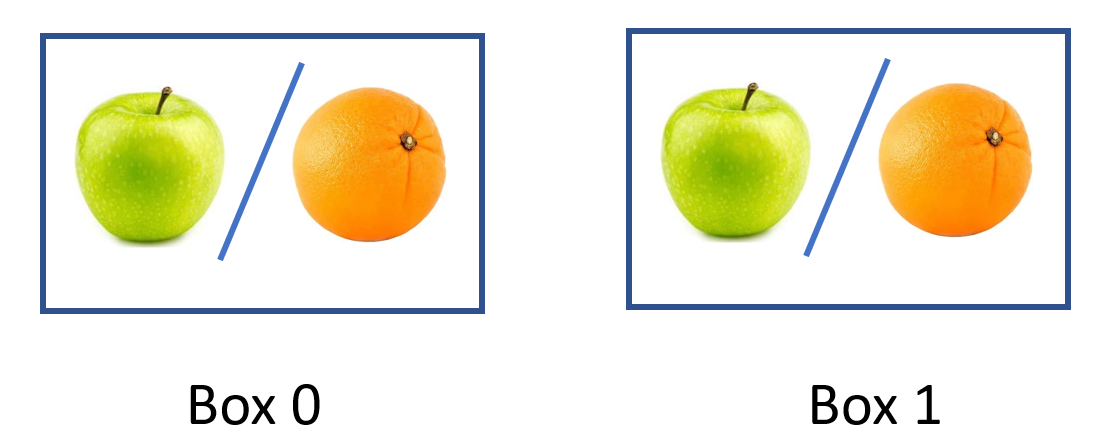
\includegraphics[width=0.4\textwidth]{deutsch_fruit}
\end{center}

Mathematically, consider a boolean function $f:\{0,1\}\to\{0,1\}$. 
The question is whether $f(0)=f(1)$ or $f(0)\ne f(1)$?
A quantum fruit-checker assumes the access to $f$ via the following quantum oracle:
\begin{equation}
U_f\ket{x,y}=\ket{x,y\oplus f(x)}, \quad x,y\in \{0,1\}.
\label{eqn:deutsch_oracle}
\end{equation}
A classical fruit-checker can only query $U_f$ in the computational basis as
\begin{equation}\label{eqn:deutsch_computationalbasis}
U_f\ket{0,0}=\ket{0,f(0)},\quad U_f\ket{1,0}=\ket{1,f(1)}.
\end{equation}
After these \emph{two} queries, we can measure qubit $1$ with a deterministic outcome, and answer whether $f(0)=f(1)$. However, a quantum fruit-checker can apply $U_f$ to a linear combination of states in the computational basis.

Let us first check that $U_f$ is unitary:

\begin{equation}
\begin{split}
\braket{x',y'|U_f^{\dag}U_f|x,y}=&\braket{x',y'\oplus f(x')|x,y\oplus f(x)}\\
=&\braket{x'|x}\braket{y'\oplus f(x')|y\oplus f(x)}\\
=&\delta_{x,x'}\delta_{y,y'}
\end{split}
\end{equation}
which gives $U_f^{\dag}U_f=I$.

 
The idea behind Deutsch's algorithm is to convert the oracle \eqref{eqn:deutsch_oracle} into a phase kickback in \cref{eqn:phase_kickback}. Take $\ket{y}=\ket{-}=\frac{1}{\sqrt{2}}(\ket{0}-\ket{1})$.
Then 
\begin{equation}\label{eqn:kickback_deutsch}
U_f \ket{x,y}=\frac{1}{\sqrt{2}}\left(\ket{x,f(x)}-\ket{x,1\oplus f(x)}\right)=(-1)^{f(x)} \ket{x,y}.
\end{equation}
Note that $\ket{y}=H X\ket{0}$, \cref{eqn:kickback_deutsch} can also be interpreted as
\begin{equation}
(I\otimes XH)U_f(I\otimes HX)\ket{x,0}=(-1)^{f(x)} \ket{x,0}.
\end{equation}
The application of $XH$ can be viewed as the step of uncomputation. Neglecting the qubit 1 which does not change before and after the application, we can focus on the first qubit only, which effectively defines a unitary
\begin{equation}
\wt{U}_f\ket{x}=(-1)^{f(x)}\ket{x}.
\end{equation}
Hence the information of $f(x)$ is stored as a phase factor ($0$ or $\pi$).
Recall that using a Hadamard gate $H\ket{0}=\ket{+}, H\ket{1}=\ket{-}$,
the quantum circuit of Deutsch's algorithm is
\begin{center}
\begin{quantikz}
\lstick{$\ket{0}$} & \gate{H} &\gate{\wt{U}_f} & \gate{H}  & \meter{}
\end{quantikz}
\end{center}
or in the commonly seen form in \cref{fig:circuit_deutsch}.
\begin{figure}[H]
\begin{center}
\begin{quantikz}
\lstick{$\ket{0}$} & \gate{H} &\gate[2][2cm]{U_f} \gateinput{$x$}\gateoutput{$x$}& \gate{H}  & \meter{}\\
\lstick{$\ket{1}$} & \gate{H} &\gateinput{$y$}\gateoutput{$y\oplus f(x)$}              & \qw 
\end{quantikz}
\end{center}
\caption{Quantum circuit for Deutsch's algorithm.}
\label{fig:circuit_deutsch}
\end{figure}
The answer is embedded in the measurement outcome of qubit $0$.
To verify this:
\begin{equation}
\begin{split}
\ket{0,1} \xrightarrow{H\otimes H}& \ket{+,-}=\frac{1}{\sqrt{2}}(\ket{0}+\ket{1})\otimes\ket{-}\\
\xrightarrow{U_f}&\frac{1}{\sqrt{2}}\left((-1)^{f(0)}\ket{0}+(-1)^{f(1)}\ket{1}\right)\otimes\ket{-}\\
\xrightarrow{H\otimes I} &\frac12\left((-1)^{f(0)}+(-1)^{f(1)}\right)\ket{0,-}\\
&+\frac12\left((-1)^{f(0)}-(-1)^{f(1)}\right)\ket{1,-}.
\end{split}
\end{equation}
So if $f(0)=f(1)$, the final state is $\pm\ket{0,-}$. Measuring qubit $0$ returns $0$ deterministically (the globally phase factor is irrelevant). Similarly if $f(0)\ne f(1)$, the final state is $\pm\ket{1,-}$. Measuring qubit $0$ returns $1$ deterministically. In summary, only \emph{one} query to $U_f$ is sufficient to answer whether the two boxes contain the same type of fruit. 
The procedure is equally counterintuitive. Note that a classical fruit checker as implemented in \cref{eqn:deutsch_computationalbasis} naturally receives the information by measuring qubit 1. 
On the other hand, Deutsch's algorithm only uses qubit 1 as a signal qubit, and all the information is retrieved by measuring qubit 0, which, at least from the classical perspective of \cref{eqn:deutsch_computationalbasis}, seems to contain no information at all!

Now we have seen that in terms of the \emph{query complexity}, a quantum fruit-checker is clearly more efficient.
However, it is a fair question how to implement the oracle $U_f$, especially in a way that somehow does not already reveal the values of $f(0),f(1)$.
We give the implementation of some cases of $U_f$ in \cref{exam:qiskit_deutsch}.
In general, proving the query complexity alone may not be convincing enough that quantum computers are better than classical computers, and the gate complexity matters. 
This will not be the last time we hide away such ``implementation details'' of quantum oracles.

\begin{rem}[Deutsch--Jozsa algorithm]
The single-qubit version of the Deutsch algorithm can be naturally generalized to the $n$-qubit version, called the Deutsch--Jozsa algorithm. Given $N=2^n$ boxes with an apple or an orange in each box, and the promise that either 1) all boxes contain the same type of fruit or 2) exactly half of the boxes contain apples and the other half contain oranges, we would like to distinguish the two cases. Mathematically, given the promise that a boolean function $f:\{0,1\}^n\to\{0,1\}$ is either a constant function (i.e., $|\set{x|f(x)=0}|=0$ or $2^n$) or a balanced function (i.e., $|\set{x|f(x)=0}|=2^{n-1}$), we would like to decide to which type $f$ belongs. We refer to \cite[Section 1.4.4]{NielsenChuang2000} for more details.
\end{rem}

\begin{exam}[Qiskit example of Deutsch's algorithm]\label{exam:qiskit_deutsch}
For $f(0)=f(1)=1$ (constant case), we can use $U_f=I\otimes X$. 
For $f(0)=0,f(1)=1$ (balanced case), we can use $U_f=\opr{CNOT}$. 
\begin{center}
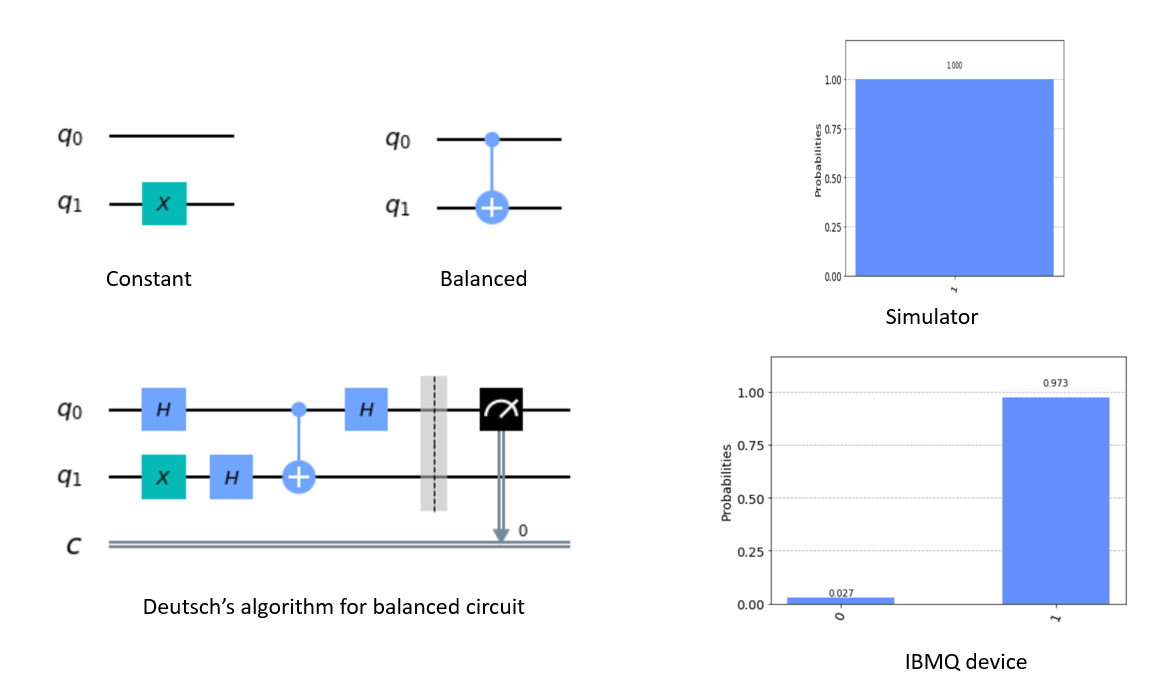
\includegraphics[width=1.0\textwidth]{deutsch_qiskit}
\end{center}
\end{exam}



\section{Unstructured search problem}\label{sec:grover}

Assume we have $N=2^{n}$ boxes, and we are given the promise that only one of the boxes contains an orange, and each of the remaining boxes contains an apple. The goal is to find the box that contains the orange.

Mathematically, given a boolean function $f:\{0,1\}^n\to\{0,1\}$ and the promise that there exists a unique marked state $x_0$ that $f(x_0)=1$, we would like to find $x_0$.
This is called an unstructured search problem. 
Classically, there is no simpler methods than opening $(N-1)$ boxes in the worst case to determine $x_0$. 

The quantum algorithm below, called Grover's algorithm, relies on access to an oracle
\begin{equation}
U_f\ket{x,y}=\ket{x,y\oplus f(x)}, \quad x\in \{0,1\}^n,y\in \{0,1\},
\label{eqn:grover_oracle}
\end{equation}
and can find $x_0$ using $\Or(\sqrt{N})$ queries.
A classical computer again can only query $U_f$ in the computational basis, and Grover's algorithm achieves a \emph{quadratic speedup} in terms of the query complexity. 

The origin of the quadratic speedup can be summarized as follows: while classical probabilistic algorithms work with probability densities, quantum algorithms work with wavefunction amplitudes, of which the square gives the probability densities. More specifically, we start from a uniform superposition of all states as the initial state
\begin{equation}
\ket{\psi_0}=\frac{1}{\sqrt{N}}\sum_{x\in[N]} \ket{x}.
\end{equation}
This state can be prepared using Hadamard gates as 
\begin{equation}
\ket{\psi_0}=H^{\otimes n}\ket{0^n}.
\end{equation}
We would like to \emph{amplify} the desired amplitude corresponding to $\ket{x_0}$ from $1/\sqrt{N}$ to $\sqrt{p}=\Omega(1)$. 
We demonstrate below that this requires $\Or(\sqrt{N})$ queries to $U_f$.
After this procedure, by measuring the final state in the computational basis, we obtain some output state $\ket{x}$. We can check whether $x=x_0$ by applying another query of $U_f$ according to $U_f \ket{x,0}=\ket{x,f(x)}$. 
The probability of obtaining $f(x)=1$ is $p$.  If $f(x)\ne 1$, we repeat the process. 
Then after $\Or(1/p)$ times of repetition, we can obtain $x_0$ with high probability.

The first step of Grover's algorithm is to turn the oracle \eqref{eqn:grover_oracle} into a phase kickback. For this we take $\ket{y}=\ket{-}$, and for any $x\in\{0,1\}^n$,
\begin{equation}
U_f\ket{x,-}=\frac{1}{\sqrt{2}}\left(\ket{x,f(x)}-\ket{x,1\oplus f(x)}\right)=(-1)^{f(x)} \ket{x,-}.
\end{equation}
Any quantum state $\ket{\psi}$ can be decomposed as
\begin{equation}
\ket{\psi}=\alpha \ket{x_0}+\beta\ket{\psi^{\perp}},
\end{equation}
where $\ket{\psi^{\perp}}$ is the component of $\ket{\psi}$ orthogonal to $\ket{x_0}$, i.e., $\braket{\psi^{\perp}|x_0}=0$. 
We have
\begin{equation}
U_f\ket{\psi}\otimes\ket{-}=(-\alpha\ket{x_0}+\beta \ket{\psi^{\perp}})\otimes\ket{-}.
\end{equation}
Here the minus sign is gained through the phase kickback.
Discarding the $\ket{-}$ which is unchanged by applying $U_f$, we obtain an $n$-qubit unitary
\begin{equation}
R_{x_0} (\alpha \ket{x_0}+\beta\ket{\psi^{\perp}})=-\alpha\ket{x_0}+\beta \ket{\psi^{\perp}}.
\end{equation}
Therefore $R_{x_0}$ is a \emph{reflection operator} across the hyperplane orthogonal to $\ket{x_0}$, i.e., the Householder reflector 
\begin{equation}
R_{x_0}=I-2\ket{x_0}\bra{x_0}.
\end{equation}

Let us write
\begin{equation}
\ket{\psi_0}=\sin (\theta/2)\ket{x_0}+\cos(\theta/2)\ket{\psi_0^{\perp}},
\end{equation}
with $\theta=2\arcsin \frac{1}{\sqrt{N}}\approx \frac{2}{\sqrt{N}}$,
and $\ket{\psi_0^{\perp}}=\frac{1}{\sqrt{N-1}}\sum_{x\ne x_0} \ket{x}$ is a normalized state orthogonal to $\ket{x_0}$. 
Then
\begin{equation}
R_{x_0}\ket{\psi_0}=-\sin(\theta/2)\ket{x_0}+\cos(\theta/2)\ket{\psi_0^{\perp}}.
\end{equation}
So $\opr{span}\{\ket{x_0},\ket{\psi_0^{\perp}}\}$ is an invariant subspace of $R_{x_0}$. 

The next key step is to consider another Householder reflector with respect to $\ket{\psi_0}$. For later convenience we add a global phase factor $-1$ (which is irrelevant to the physical outcome):
\begin{equation}
R_{\psi_0}=-(I-2\ket{\psi_0}\bra{\psi_0}).
\end{equation}

Direct computation shows 
\begin{equation}
\begin{split}
R_{\psi_0}R_{x_0}\ket{\psi_0}=&R_{\psi_0}(\ket{\psi_0}-2\sin(\theta/2)\ket{x_0})\\
=&(\ket{\psi_0}-4\sin^2(\theta/2)\ket{\psi_0})+2\sin(\theta/2)\ket{x_0}\\
=&\sin (\theta/2) (3-4\sin^2 (\theta/2))\ket{x_0}+ 
\cos (\theta/2)(1-4\sin^2 (\theta/2))\ket{\psi_0^{\perp}}\\
=& \sin(3\theta/2)\ket{x_0}+\cos(3\theta/2)\ket{\psi_0^{\perp}}.
\end{split}
\end{equation}
So define $G=R_{\psi_0}R_{x_0}$ as the product of the two reflection operators (called the Grover operator), then it amplifies the angle from $\theta/2$ to $3\theta/2$.
The geometric picture is in fact even clearer in \cref{fig:grover_rotation} and the conclusion can be observed without explicit computation.

\begin{figure}[H]
\begin{center}
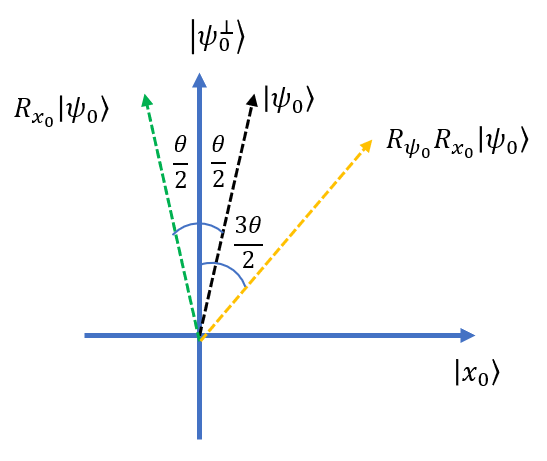
\includegraphics[width=0.4\textwidth]{grover_rotation}
\end{center}
\caption{Geometric interpretation of one Grover iteration.}
\label{fig:grover_rotation}
\end{figure}

Applying the Grover operator $k$ times, we obtain 
\begin{equation}\label{eqn:grover_k}
G^k \ket{\psi_0}=\sin((2k+1)\theta/2)\ket{x_0}+\cos((2k+1)\theta/2)\ket{\psi_0^{\perp}}.
\end{equation}
So for $\sin((2k+1)\theta/2)\approx 1$, we need $k\approx \frac{\pi}{2\theta}-\frac{1}{2}\approx \frac{\sqrt{N}\pi}{4}$.
This proves that Grover's algorithm can solve the unstructured search problem with $\Or(\sqrt{N})$ queries to $U_f$.

Another derivation of the Grover method is to focus on the operator, instead of the initial vector $\ket{\psi_0}$ at each step of the calculation.
In the orthonormal basis $\mc{B}=\{\ket{x_0},\ket{\psi_0^{\perp}}\}$, the matrix representation of the reflector $R_{x_0}=I-2\ket{x_0}\bra{x_0}$ is
\begin{equation}
[R_{x_0}]_{\mc{B}}=\begin{pmatrix}
-1 & 0 \\
0 & 1
\end{pmatrix}.
\end{equation}
The matrix representation for the Grover diffusion operator $R_{\psi_0}=2\ket{\psi_0}\bra{\psi_0}-I$ is
\begin{equation}
[R_{\psi_0}]_{\mc{B}}=\begin{pmatrix}
2a^2-1 & 2a\sqrt{1-a^2} \\
2a\sqrt{1-a^2} & 1-2a^2
\end{pmatrix}=\begin{pmatrix}
-\cos \theta & \sin\theta \\
\sin\theta & \cos\theta
\end{pmatrix}.
\end{equation}
Here $\sin(\theta/2)=a=1/\sqrt{N}$. Therefore for the matrix representation of the Grover iterate $G=R_{\psi_0}R_{x_0}$ is
\begin{equation}
\label{eqn:grover_step_matrix}
[G]_{\mc{B}}=\begin{pmatrix}
\cos \theta & \sin\theta \\
-\sin\theta & \cos\theta
\end{pmatrix},
\end{equation}
i.e., $G$ is a rotation matrix restricted to the two-dimensional space $\mc{H}=\opr{span}\mc{B}$.

The initial vector satisfies 
\begin{equation}
[\ket{\psi_0}]_{\mc{B}}=\begin{pmatrix}
\sin(\theta/2)\\
\cos(\theta/2)
\end{pmatrix},
\end{equation}
so Grover's search can be applied as before, via $G^k$ for $k\approx \frac{\pi\sqrt{N}}{4}$  times.


To draw the quantum circuit of Grover's algorithm, we need an implementation of $R_{\psi_0}$. 
Note that
\begin{equation}
R_{\psi_0}=H^{\otimes n}(2\ket{0^n}\bra{0^n}-I)H^{\otimes n}.
\end{equation}
This can be implemented via the following circuit using one ancilla qubit:
\begin{displaymath}
\begin{quantikz}
\lstick{$\ket{-}$}& \gate{X} & \targ{} & \qw & \qw\\
\lstick{$\ket{\psi}$}&  \gate{H^{\otimes n}}& \octrl{-1} & \gate{H^{\otimes n}} & \qw
\end{quantikz}
\end{displaymath}
Here the controlled-NOT gate is an $n$-qubit controlled-$X$ gate, and is only active if the system qubits are in the $0^n$ state.
Discarding the signal qubit, we obtain and implementation of $R_{\psi_0}$.
Since the signal qubit $\ket{-}$ only changes up to a sign, it can be reused for both $R_{\psi_0}$ and $R_{x_0}$.

The reflector $R_{\psi_0}$ can also be implemented without using the ancilla qubit as (use a 3-qubit system as an example)
\begin{figure}[H]
\begin{displaymath}
\begin{quantikz}
&  \gate{H}& \gate{X}&\gate{Z} & \gate{X}&\gate{H} & \qw\\
&  \gate{H}& \gate{X}&\ctrl{-1} & \gate{X}&\gate{H} & \qw\\
&  \gate{H}& \gate{X}&\ctrl{-1} & \gate{X}&\gate{H} & \qw
\end{quantikz}
\end{displaymath}
\caption{Implementing $R_{\psi_0}$ for a three qubit system.}
\label{fig:rpsi0}
\end{figure}




\begin{rem}[Multiple marked states] The Grover search algorithm can be naturally generalized to the case when there are $M>1$ marked states.
The query complexity is $\Or(\sqrt{N/M})$.
\end{rem}

\begin{exam}[Qiskit for Grover's algorithm]
\url{https://qiskit.org/textbook/ch-algorithms/grover.html}
\end{exam}

\section{Amplitude amplification}\label{sec:amplitudeamplification}

Grover's algorithm is not restricted to the problem of unstructured search.
One immediate application is called amplitude amplification (AA), which is used ubiquitously as a subroutine to achieve quadratic speedups.

Let \(\ket{\psi_0}\) be prepared by an oracle $U_{\psi_0}$, i.e., $U_{\psi_0}\ket{0^n}=\ket{\psi_0}$.
We have the knowledge that
\begin{equation}
\ket{\psi_0}=\sqrt{p_0} \ket{\psi_{\mathrm{good}}}+\sqrt{1-p_0} \ket{\psi_{\mathrm{bad}}},
\end{equation}
and $p_0\ll 1$. Here $\ket{\psi_{\mathrm{bad}}}$ is an orthogonal state to the desired state $\ket{\psi_{\mathrm{good}}}$.
We cannot get access to $\ket{\psi_{\mathrm{good}}}$ directly, but would like to obtain a state that has a large overlap with $\ket{\psi_{\mathrm{good}}}$, i.e., amplify the amplitude of $\ket{\psi_{\mathrm{good}}}$.



In the problem of unstructured search, $\ket{\psi_{\mathrm{good}}}=\ket{x_0}$,
and $p_0=1/N$. 
Although we do not have access to the answer $\ket{x_0}$, we assume access to the reflection oracle $R_{x_0}$.
Here we also assume access to the reflection oracle
\begin{equation}
R_{\mathrm{good}}=1-2\ket{\psi_{\mathrm{good}}}\bra{\psi_{\mathrm{good}}}.
\end{equation}
From $U_{\psi_0}$, we can construct the reflection with respect to the initial state
\begin{equation}\label{eqn:R_psi0}
R_{\psi_0}=2\ket{\psi_0}\bra{\psi_0}-I=U_{\psi_0}(2\ket{0^n}\bra{0^n}-I)U^{\dag}_{\psi_0}
\end{equation}
via the $n$-qubit controlled-$X$ gate.
So following exactly the same procedure as the unstructured search problem, we can construct the Grover iterate
\begin{equation}
G=R_{\psi_0}R_{\mathrm{good}}.
\end{equation}
Applying $G^k$ to $\ket{\psi_0}$ for some $k=\Or(1/\sqrt{p_0})$, we obtain a state that has $\Omega(1)$ overlap with $\ket{\psi_{\mathrm{good}}}$.

\begin{exam}[Reflection with respect to signal qubits]
  \label{exam:ref_signal}
One common scenario is that the implementation of $U_{\psi_0}$ requires $m$ ancilla qubits (also called signal qubits), i.e.,
\begin{equation}
U_{\psi_0}\ket{0^m}\ket{0^n}=\sqrt{p_0}\ket{0^m}\ket{\psi_0}+\sqrt{1-p_0}\ket{\perp},
\label{eqn:Upsi0_mark}
\end{equation}
where $\ket{\perp}$ is some orthogonal state satisfying
\begin{equation}
(\Pi\otimes I_n)\ket{\perp}=0, \quad \Pi=\ket{0^m}\bra{0^m}.
\end{equation}
Therefore
\begin{equation}
\ket{\psi_{\mathrm{good}}}=\ket{0^m}\ket{\psi_0}, \quad \ket{\psi_{\mathrm{bad}}}=\ket{\perp}.
\end{equation}
This setting is special since the ``good'' state can be verified by measuring the ancilla qubits after applying $U_{\psi_0}$ in \cref{eqn:Upsi0_mark}, and post-select the outcome $0^m$.
In particular, the expected number of measurements needed to obtain $\ket{\psi_{\mathrm{good}}}$ is $1/p_0$.

In order to employ the AA procedure, we first note that the reflection operator can be simplified as
\begin{equation}
R_{\mathrm{good}}=(1-2\ket{0^m}\bra{0^m})\otimes I_n=(1-2\Pi)\otimes I_n.
\end{equation}
This is because $\ket{\psi_{\mathrm{good}}}$ can be entirely identified by measuring the ancilla qubits. 
Meanwhile 
\begin{equation}
R_{\psi_0}=U_{\psi_0}(2\ket{0^{m+n}}\bra{0^{m+n}}-I)U^{\dag}_{\psi_0}.
\end{equation}
Let $G=R_{\psi_0}R_{\mathrm{good}}$, and applying $G^k$ to $\ket{\psi_0}$ for some $k=\Or(1/\sqrt{p_0})$ times, we obtain a state that has $\Omega(1)$ overlap with $\ket{\psi_{\mathrm{good}}}$. 
This achieves the desired quadratic speedup.
\end{exam}


\begin{exam}[Amplitude damping] Assuming access to an oracle in \cref{eqn:Upsi0_mark}, where $p_0$ is large, we can easily dampen the amplitude to any number $\alpha\le \sqrt{p_0}$.
% We introduce an additional signal qubit, and for simplicity let us assume $m=1$.
% Then  \cref{eqn:Upsi0_mark} becomes
% \begin{equation}
% (I\otimes U_{\psi_0})\ket{0}\ket{0}\ket{0^n}=\ket{0}\sqrt{p_0}\ket{0}\ket{\psi_0}+\sqrt{1-p_0}\ket{\perp}.
% \end{equation}
% Now for $\ket{b}=b_0\ket{0}+b_1\ket{1}$, define the controlled rotation
% \begin{equation}\label{eqn:controlled_rotation_simple}
% \opr{CR}\ket{0}\ket{b}=b_0 (\cos \theta \ket{0}+\sin \theta\ket{1})\ket{0}+b_1\ket{1},
% \end{equation}
% we have
% \begin{equation}
% (\opr{CR}\otimes I_n)(I\otimes U_{\psi_0})\ket{0}\ket{0}\ket{0^n}=\sqrt{p_0}\cos \theta\ket{0}\ket{0}\ket{\psi_0}+\sqrt{1-p_0}\ket{\perp'}.
% \end{equation}
% Then just choose $\sqrt{p_0}\cos \theta=\alpha$.
% 
% When the number of ancilla qubits $m>1$, we need to replace the controlled rotation by the multi-qubit controlled rotation.

We introduce an additional signal qubit. Then  \cref{eqn:Upsi0_mark} becomes
\begin{equation}
(I\otimes U_{\psi_0})\ket{0}\ket{0}\ket{0^n}=\ket{0}\sqrt{p_0}\ket{0}\ket{\psi_0}+\sqrt{1-p_0}\ket{\perp}.
\end{equation}
Define a single qubit rotation operation as 
\begin{equation}\label{eqn:controlled_rotation_simple}
R_{\theta}\ket{0}=\cos \theta \ket{0}+\sin \theta\ket{1},
\end{equation}
and we have
\begin{equation}
\begin{split}
&(R_{\theta}\otimes I_{m+n})(I\otimes U_{\psi_0})\ket{0}\ket{0^m}\ket{0^n}\\
=&\cos \theta\ket{0}(\sqrt{p_0}\ket{0^m}\ket{\psi_0}+\sqrt{1-p_0}\ket{\perp'})+
\sin \theta\ket{1}(\sqrt{p_0}\ket{0^m}\ket{\psi_0}+\sqrt{1-p_0}\ket{\perp'})\\
:=&\sqrt{p_0}\cos \theta\ket{0}\ket{0^m}\ket{\psi_0}+\sqrt{1-p_0\cos^2\theta}\ket{\perp'}.
\end{split}
\end{equation}
Here $(\ket{0^{m+1}}\bra{0^{m+1}}\otimes I_n)\ket{\perp'}=0$.
We only need to choose $\sqrt{p_0}\cos \theta=\alpha$. 

\end{exam}


\section{Lower bound of query complexity*}\label{sec:lowerbound_grover}

Recall that the unstructured search problem tries to find a marked state $x_0\in[N]$, using a reflection oracle
\begin{equation}
R_{x_0}=I-2\ket{x_0}\bra{x_0}.
\end{equation}
Grover's algorithm can find $x_0$ with constant probability (e.g. at least $1/2$) by making $\Or(\sqrt{N})$ times querying $R_{x_0}$. 
It turns out that this is \emph{asymptotically optimal}, i.e., no quantum algorithm can perform this task using fewer than $\Omega(\sqrt{N})$ access to $R_{x_0}$.

Any quantum search algorithm that starts from a universal initial state $\ket{\psi_0}$ and queries $R_{x_0}$ for $k$ steps can be written in the following form:
\begin{equation}
\ket{\psi^{x_0}_k}=\mc{U}^{x_0}_k\ket{\psi_0}=U_kR_{x_0}\cdots U_2R_{x_0} U_1R_{x_0}\ket{\psi_0},
\end{equation}
for some unitaries $U_1,\ldots,U_k$.
For simplicity we assume no ancilla qubits are used, and the proof can be generalized to the case in the presence of ancilla qubits.
The superscript $x_0$ indicates that the state depends on the marked state $x_0$.
Specifically, by ``solving'' the search problem, it means that there exists a $k$ so that for each marked state $x_0$, 
\begin{equation}\label{eqn:def_grover_success}
|\braket{\psi^{x_0}_k|x_0}|^2\ge \frac12.
\end{equation}
In other words, measuring $\ket{\psi^{x_0}_k}$ in the computational basis, the probability of obtaining $\ket{x_0}$ is at least $1/2$. 

To prove the lower bound, we compare the action of $\mc{U}^{x_0}_k$ with another ``fake algorithm'' $\mc{U}_k$, defined as
\begin{equation}
\ket{\psi_k}=\mc{U}_k\ket{\psi_0}=U_k\cdots U_2 U_1\ket{\psi_0}.
\end{equation}
In particular,  $\ket{\psi_k}$ does not involve any information of the solution $x_0$ and therefore cannot possibly solve the search problem.


For a set of vectors $\{f^{x_0}\}_{x_0\in [N]}$, and each $f^{x_0}\in \CC^N$, we will extensively use the following discrete $\ell_2$-norm:
\begin{equation}
\norm{f}_{\ell_2}:=\left(\sum_{x_0\in[N]} \norm{f^{x_0}}\right)^{\frac12}.
\end{equation}
In particular, we have the following triangle inequality
\begin{equation}
\norm{f}_{\ell_2}-\norm{g}_{\ell_2}\le\norm{f+g}_{\ell_2}\le\norm{f}_{\ell_2}+\norm{g}_{\ell_2}.
\end{equation}

The proof contains two steps. First, we show that the true solution and the fake solution differs significantly, in the sense that 
\begin{equation}\label{eqn:dk_lowerbound}
D_k:=\sum_{x_0\in[N]}\norm{\ket{\psi^{x_0}_k}-\ket{\psi_k}}^2=\Omega(N).
\end{equation}
Second, we prove that (define $D_0=0$):
\begin{equation}
D_k\le 4k^2, \quad k\ge 0.
\label{eqn:grover_dk}
\end{equation}
Therefore to satisfy \cref{eqn:dk_lowerbound}, we must have $k=\Omega(\sqrt{N})$.

In the first step, since multiplying a phase factor $e^{\I \theta}$ to $\ket{\psi^{x_0}_k}$ does not have any physical consequences, we may choose a particular phase $\theta$ so that \cref{eqn:def_grover_success} becomes
\begin{equation}
\braket{\psi^{x_0}_k|x_0}\ge \frac{1}{\sqrt{2}}.
\end{equation}
Therefore
\begin{equation}
\norm{\ket{\psi^{x_0}_k}-\ket{x_0}}^2= 2-2\braket{\psi^{x_0}_k|x_0}\le 2-\sqrt{2}.
\end{equation}
This means that
\begin{equation}
\sum_{x_0\in[N]}\norm{\ket{\psi^{x_0}_k}-\ket{x_0}}^2\le 2N-\sqrt{2}N.
\label{eqn:search_correct_cor}
\end{equation}

On the other hand, for the ``fake algorithm'', using the Cauchy-Schwarz inequality,
\begin{equation}
\sum_{x_0\in[N]}\norm{\ket{\psi_k}-\ket{x_0}}^2\ge 2N-2\sum_{x_0\in[N]}|\braket{x_0|\psi}|\ge2N-2\sqrt{N} \sum_{x_0\in[N]}|\braket{x_0|\psi}|^2=2N-2\sqrt{N}.
\label{eqn:search_fake_cor}
\end{equation}
This violates the bound in \cref{eqn:search_correct_cor}, and the fake algorithm cannot solve the search problem for arbitrarily large $k$.

So from \cref{eqn:search_correct_cor,eqn:search_fake_cor}, and the triangle inequality, we have
\begin{equation}
\begin{split}
D_k=\sum_{x_0\in[N]}\norm{\ket{\psi^{x_0}_k}-\ket{\psi_k}}^2&=\sum_{x_0\in[N]}\norm{(\ket{\psi^{x_0}_k}-\ket{x_0})-(\ket{\psi_k}-\ket{x_0})}^2\\
&\ge \left(\sqrt{\sum_{x_0\in[N]}\norm{\ket{\psi_k}-\ket{x_0}}^2}-\sqrt{\sum_{x_0\in[N]}\norm{\ket{\psi^{x_0}_k}-\ket{x_0}}^2}\right)^2\\
&\ge \left(\sqrt{2N-2\sqrt{N}}-\sqrt{2N-\sqrt{2}N}\right)^2\\
&=\Omega(N). 
\end{split}
\end{equation}
This proves \cref{eqn:dk_lowerbound}.
In other words, the true solution and the fake solution must be well separated in $\ell_2$-norm.


In the second step, we prove \cref{eqn:grover_dk} inductively. 
Clearly  \cref{eqn:grover_dk} is true for $k=0$. 
Assume this is true, then
\begin{equation}
\begin{split}
D_{k+1}&=\sum_{x_0\in[N]}\norm{\ket{\psi^{x_0}_{k+1}}-\ket{\psi_{k+1}}}^2\\
&=\sum_{x_0\in[N]}\norm{U_{k+1}R_{x_0}\ket{\psi^{x_0}_{k}}-U_{k+1}\ket{\psi_{k}}}^2\\
&=\sum_{x_0\in[N]}\norm{R_{x_0}\ket{\psi^{x_0}_{k}}-\ket{\psi_{k}}}^2\\
&=\sum_{x_0\in[N]}\norm{R_{x_0}(\ket{\psi^{x_0}_{k}}-\ket{\psi_{k}})+(R_{x_0}-I)\ket{\psi_{k}}}^2\\
&\le \left(\sqrt{\sum_{x_0\in[N]}\norm{R_{x_0}(\ket{\psi^{x_0}_{k}}-\ket{\psi_{k}})}^2}+\sqrt{\sum_{x_0\in[N]}\norm{(R_{x_0}-I)\ket{\psi_{k}}}^2}\right)^2.
\end{split}
\end{equation}
The last inequality uses the triangle inequality of the discrete $\ell_2$-norm.
Note that
\begin{equation}
\sqrt{\sum_{x_0\in[N]}\norm{(R_{x_0}-I)\ket{\psi_{k}}}^2}=\sqrt{4\sum_{x_0\in[N]}\abs{\braket{x_0|\psi_k}}^2}=2,
\end{equation}
and 
\begin{equation}
\sqrt{\sum_{x_0\in[N]}\norm{R_{x_0}(\ket{\psi^{x_0}_{k}}-\ket{\psi_{k}})}^2}=\sqrt{\sum_{x_0\in[N]}\norm{\ket{\psi^{x_0}_{k}}-\ket{\psi_{k}}}^2}=\sqrt{D_k},
\end{equation}
we have
\begin{equation}
\sqrt{D_{k+1}}\le \sqrt{D_k}+2\le 2(k+1), 
\end{equation}
which finishes the induction.

Finally, combining the lower bound \cref{eqn:dk_lowerbound,eqn:grover_dk}, we find that the necessary condition to solve the unstructured search problem is $4k^2=\Omega(N)$, or $k=\Omega(\sqrt{N})$.


\begin{rem}[Implication for amplitude amplification]
Due to the close relation between unstructred search and amplitude amplification, it means that given a state $\ket{\psi}$ of which the amplitude of the ``good'' component is $\alpha\ll 1$, no quantum algorithms can amplify the amplitude to $\Omega(1)$ using $o(\alpha^{-\frac12})$ queries to the reflection operators.
\end{rem}

\vspace{2em}

\begin{exer}
In Deutsch's algorithm, demonstrate why not assuming access to an oracle $V_f:\ket{x}\mapsto\ket{f(x)}$.
\end{exer}

\begin{exer}
For all possible mappings $f:\{0,1\}\to\{0,1\}$, draw the corresponding quantum circuit to implement $U_f:\ket{x,0}\mapsto\ket{x,f(x)}$.
\end{exer}

\begin{exer}
Prove \cref{eqn:grover_k}.
\end{exer}

\begin{exer}
Draw the quantum circuit for \cref{eqn:R_psi0}.
\end{exer}

\begin{exer}
Prove that when ancilla qubits are used, the complexity of the unstructured search problem is still $\Omega(\sqrt{N})$.
\end{exer}
